	\section{Simulations}
	To demonstrate the previous results, we simulate random graphs from a SBM with parameters.
	\begin{equation*}
	B = \begin{bmatrix}
	.42 & .2 \\
	.2 & .7 
	\end{bmatrix}
	,\qquad \rho = \begin{bmatrix}
	.5 & .5
	\end{bmatrix}
	\end{equation*}
	
	From this model we sample $M$ Adjacency Matrices with $N$ vertices to calculate both $\bar{A}$ and $\hat{P}$.  With these estimators for $P$, we calculate the mean squared error of each block region in the model, and compare these with our predictions.
	
	\begin{figure}[!htb]
		\centering
		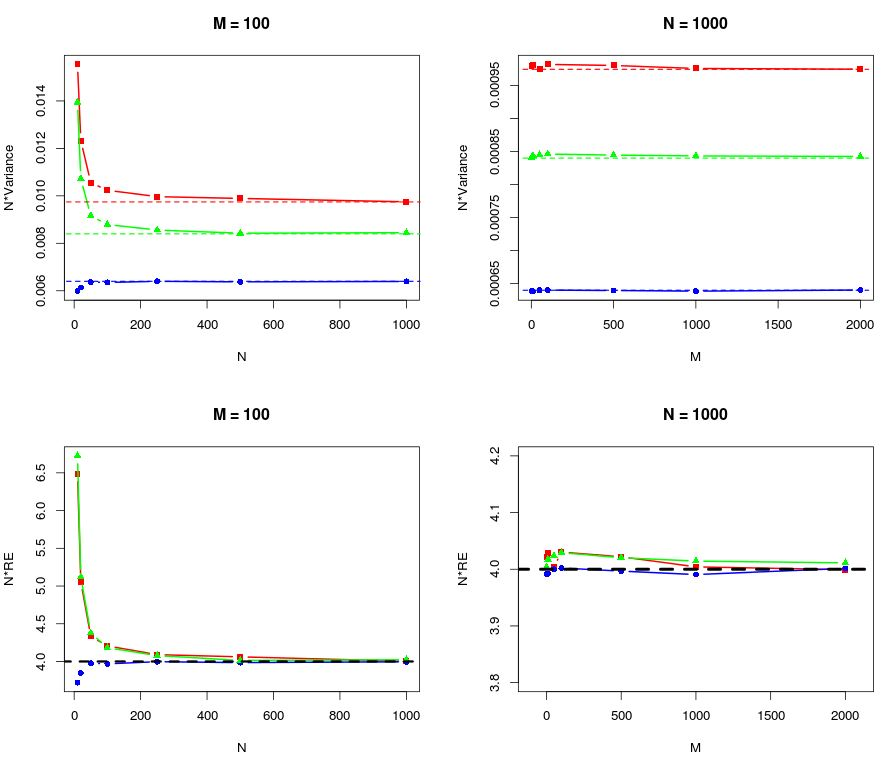
\includegraphics[width=16cm]{Var_RE.JPG}
		\caption{N*Variance$(\hat{P})$ and RE, dotted lines represent the predictions and each color represents unique values within the true $P \in \{.2,.42,.7\}$ }
		\label{fig:plot1}
	\end{figure}
	\newpage
	We now examine simulations where we vary the $\rho$ vector for the SBM with the following parameters:
	
		\begin{equation*}
		B = \begin{bmatrix}
		.42 & .2 \\
		.2 & .7 
		\end{bmatrix}
		,\qquad N = 500,\qquad M = 100
		\end{equation*}
	
	\begin{figure}[!htb]
		\centering
		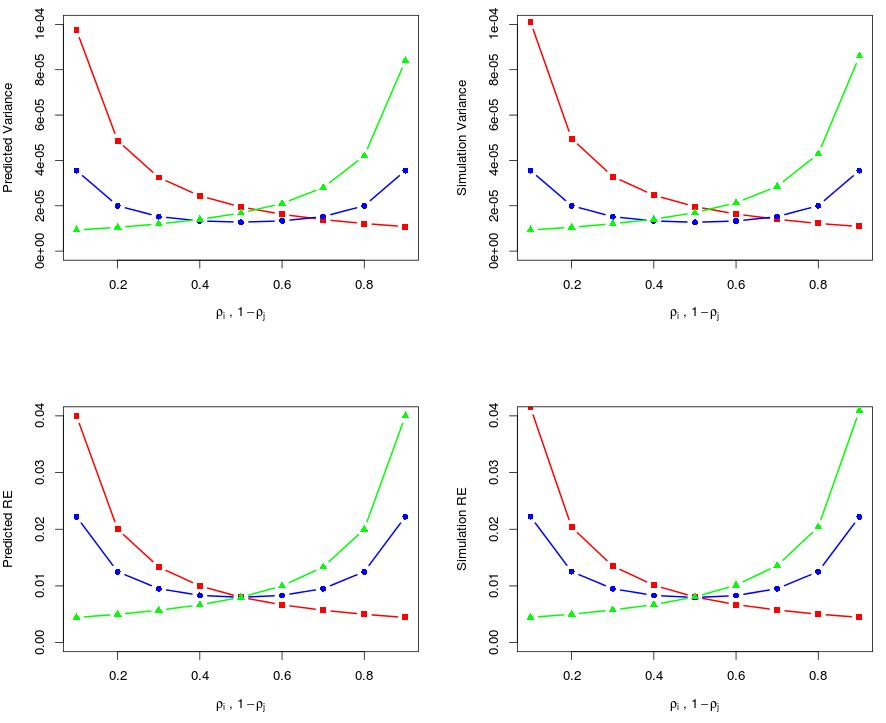
\includegraphics[width=16cm]{PI.JPG}
		\caption{N*Variance$(\hat{P})$ and RE, plots on the left are Predicted values corresponding to the right plot and each color represents unique values within the true $P \in \{.2,.42,.7\}$ }
		\label{fig:plot1}
	\end{figure}
	\newpage